% vim: set spell spelllang=es syntax=tex :

\section{OpenMP: Open Multi-Processing}

\label{mt_openmp}

\emph{OpenMP} es una API de bibliotecas y directivas al compilador para la
definición de paralelismo de alto nivel para sistemas \emph{MIMD} de memoria
compartida en \emph{C}, \emph{C++} y \emph{Fortran} \cite{ompWeb}. Es una API
abierta, publicada y definida por el consorcio \emph{OpenMP Architecture Review
Board} (o \emph{OpenMP ARB}). El consorcio está compuesto por representantes de
las industrias del hardware y software. Sus miembros permanentes son \emph{AMD},
\emph{ARM}, \emph{CRAY}, \emph{Fujitsu}, \emph{HPE}, \emph{IBM}, \emph{Intel},
\emph{Micron}, \emph{NEC}, \emph{NVIDIA}, \emph{Oracle}, \emph{Red Hat}, y
\emph{Texas Instruments} y, sus miembros temporales incluyen al centro de
cómputo Barcelona, la \emph{NASA} y \emph{cOMPunity}, entre otros \cite{ompWeb}.
La primera publicación de \emph{OpenMP} fue su versión para \emph{Fortran} en
octubre de 1997, las especificaciones para \emph{C} y \emph{C++} fueron
publicadas en octubre de 1998.

\emph{OpenMP} permite la creación de regiones paralelas, secciones críticas,
tareas y puntos de sincronización, simplemente marcando un bloque de código
con unas pocas directivas al compilador. Originalmente implementaba sólo el
modelo de \emph{fork and join}, pero a partir de la versión 3.0 se agregó el
modelo de tareas explícitas \cite{openmp08}. Ambos modelos fueron utilizados
para la implementación del sistema.

El modelo de \emph{fork and join} fue propuesto por primera vez en
\cite{conway1963}. En este modelo, la ejecución del programa está a cargo de un
solo hilo al comienzo de la ejecución y durante sus secciones secuenciales. El
hilo inicial es llamado hilo principal. Cuando se encuentra una región de
trabajo compartido (o \emph{worksharing region}) de $N$ tareas, el hilo
principal crea $N-1$ nuevos hilos. Cada hilo (incluido el hilo principal)
ejecuta una de las $N$ tareas. Esta etapa es llamada \emph{fork}. El hilo
principal no continúa la ejecución secuencial hasta que no han finalizado todas
las tareas paralelas. A esta sincronización se la llama \emph{join}. La figura
\ref{conway} muestra un ejemplo en el cual se crean dos tareas paralelas.
\emph{OpenMP} extiende el modelo permitiendo que la cantidad de hilos sea menor
que la cantidad de tareas, cuando esto sucede, las tareas sin hilo asignado son
colocadas en una lista de tareas en espera. Cuando un hilo termina de ejecutar
una tarea, si hay tareas esperando en la lista de tareas en espera, toma una y
la ejecuta. El modelo de \emph{fork and join} puede aplicarse tanto para
paralelismo de tareas como de datos.

\begin{figure}[!htb]

	\centering

	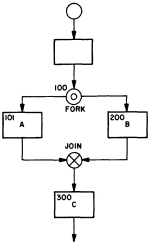
\includegraphics[height=0.25\textheight]{img/conway.pdf}

	\caption{Descripción original del modelo de \emph{fork and join}
	presentado por Melvin Conway en 1963 \cite{conway1963}.}

	\label{conway}

\end{figure}

Dado que la creación de hilos suele ser una operación costosa, la mayoría de las
implementaciones de \emph{OpenMP} suelen no destruir los hilos creados durante
el \emph{fork}, sino que se mantienen inactivos para ser reutilizados cuando se
encuentre otra región de trabajo compartido.

El segundo modelo implementado en \emph{OpenMP} a partir de la versión 3.0 es el
de tareas. Este modelo permite la creación de nuevas tareas explícitas dentro de
una región de trabajo compartido. Cuando se encuentra un área de trabajo
compartido, se crean una o más tareas implícitas y $N$ hilos de ejecución. Al
igual que el modelo de \emph{fork and join} extendido, la cantidad de hilos
puede ser menor que la cantidad de tareas, pero también puede ser mayor. Durante
la ejecución una tarea, ésta puede crear nuevas tareas explícitas a través de la
directiva \emph{task}. Si hay hilos de ejecución libres, la nueva tarea sera
asignada a uno de ellos, sino es colocada en una lista de tareas en espera.
Cuando un hilo termina de ejecutar una tarea, toma otra de la lista de tareas en
espera de tareas o espera. Sólo se destruyen los hilos al terminar la ejecución
de todas las tareas y salir de la región de trabajo compartido.

\subsubsection{Directivas de OpenMP}

El control de la creación de hilos y tareas en \emph{OpenMP} se realiza a través
de directivas al compilador. En esta sección mencionaremos aquellas utilizadas
por el sistema propuesto. En \emph{C} y \emph{C++} todas las directivas toman la
forma de \textbf{\#pragma omp DIRECTIVA [OPCIONES]}.

\begin{itemize}

	\item	La directiva más utilizada es \emph{parallel [num\_threads(N)]},
		ésta define una región de trabajo paralelo y crea $N-1$ hilos de
		ejecución (si no se incluye \emph{num\_threads(N)}, la cantidad
		de hilos se establece por medio de una variable global, y en
		caso de que ésta no esté definida, dependerá de la
		implementación). Cada hilo ejecutará una tarea definida por el
		bloque inmediato a la directiva, implementando el modelo
		\emph{fork and join}.

	\item	Si se desea que un bloque sea ejecutado sólo por un hilo se pueden
		utilizar las directivas \emph{single} y \emph{master}. Éstas
		asegurarán que el bloque inmediato sea ejecutado sólo por uno de
		los hilos del grupo. En el caso de la directiva \emph{single},
		cualquiera de los hilos del grupo podrá ser elegido para
		ejecutar el bloque, mientras que en el caso de \emph{master},
		sólo el hilo principal del grupo lo ejecutará.

	\item	Para la creación de una región de trabajo compartido bajo el
		modelo de tareas, se utiliza la directiva \emph{parallel
		num\_threads(N)} para crear los $N$ hilos de ejecución, seguida
		de la directiva \emph{master} o \emph{single} para que sólo el
		hilo principal ejecute la tarea que crea las primeras tareas de
		la región de trabajo compartido.
	
	\item	Para la creación de cada tarea se debe utilizar la directiva
		\emph{task} seguida del bloque que contiene el código a ejecutar
		por la tarea.

	\item	Si un hilo necesita esperar la finalización de las tareas que
		creó, antes de continuar su ejecución, puede utilizar la
		directiva \emph{taskwait}.

	\item	Si se desea que cada hilo ejecute una tarea con código distinto se
		debe utilizar la directiva \emph{parallel sections
		num\_threads(N)}. El bloque inmediato debe contener a su vez
		bloques precedidos por la directiva \emph{section}. Al igual que
		\emph{parallel}, esta directiva define una región de trabajo
		paralelo de $N$ hilos, pero el código de cada tarea está
		definido por los bloques inmediatos a las directivas
		\emph{section}. En caso de que se creen más hilos que las tareas
		definidas, los hilos sobrantes no ejecutarán. El modelo
		implementado por esta directiva es \emph{fork and join}.

	\item	Para definir secciones críticas se pueden utilizar las directivas
		\emph{critical [NOMBRE]} y \emph{atomic}. La primera permite
		definir un bloque de complejidad arbitraria como sección
		crítica, e incluso permite definir bloques distintos como la
		misma sección crítica si comparten el mismo nombre. La segunda
		directiva sólo acepta bloques en los cuales se realiza una
		operación aritmética simple, y resulta en una implementación
		más eficiente.

\end{itemize}

En la figura \ref{directivas} se muestra un código de ejemplo del uso de las
directivas presentadas junto con un diagrama mostrando una posible secuencia
de ejecución.

\begin{figure}[!htb]

	\centering

	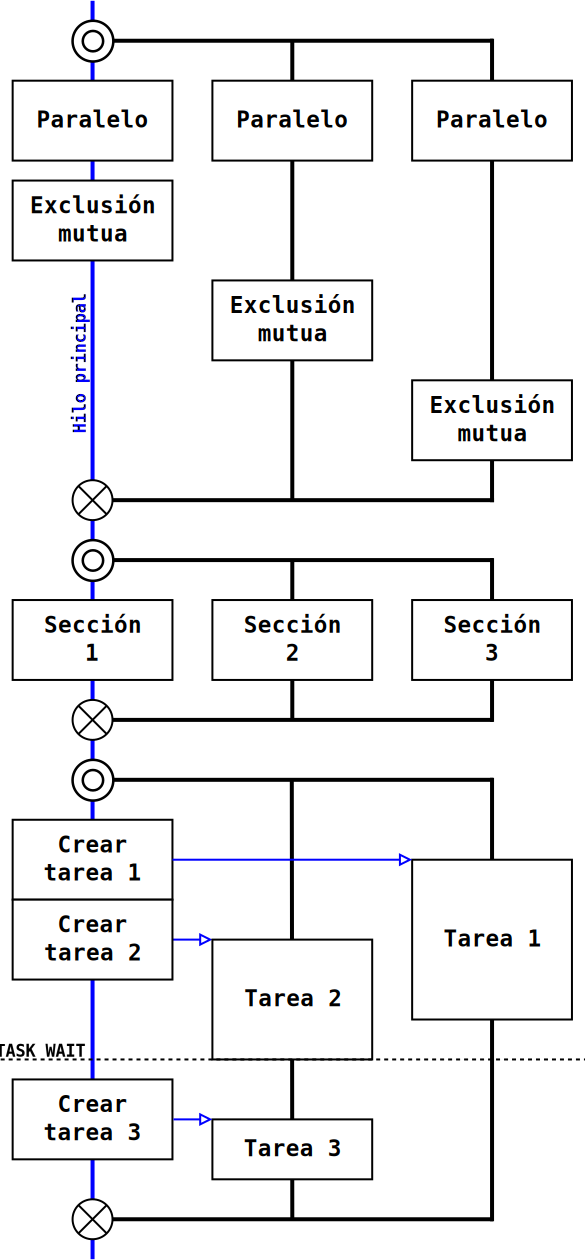
\includegraphics[height=0.40\textheight]{img/directivasOMP.pdf}
	\includegraphics{img/codigoDirectivasOMP.pdf}

	\caption{Código de ejemplo de uso de directivas de \emph{OpenMP} y
	posible secuencia de ejecución.}

	\label{directivas}

\end{figure}
